\documentclass{article}
\usepackage[utf8]{inputenc}

\title{Trajectories of Dirichlet Processes and Convergence}
\author{lucasilva11, Caicai Chen, Paolo Ceriani }
\date{May 2021}

\usepackage{algorithm}
\usepackage{algorithmic}
\usepackage[margin=1in]{geometry}

\usepackage{listings}

\lstset{breaklines=true}

\makeatletter
\newenvironment{breakablealgorithm}
  {% \begin{breakablealgorithm}
   \begin{center}
     \refstepcounter{algorithm}% New algorithm
     \hrule height.8pt depth0pt \kern2pt% \@fs@pre for \@fs@ruled
     \renewcommand{\caption}[2][\relax]{% Make a new \caption
       {\raggedright\textbf{\fname@algorithm~\thealgorithm} ##2\par}%
       \ifx\relax##1\relax % #1 is \relax
         \addcontentsline{loa}{algorithm}{\protect\numberline{\thealgorithm}##2}%
       \else % #1 is not \relax
         \addcontentsline{loa}{algorithm}{\protect\numberline{\thealgorithm}##1}%
       \fi
       \kern2pt\hrule\kern2pt
     }
  }{% \end{breakablealgorithm}
     \kern2pt\hrule\relax% \@fs@post for \@fs@ruled
   \end{center}
  }
\makeatother

\usepackage{stmaryrd}
\usepackage{subcaption}
\usepackage{graphicx}
\usepackage{amssymb}
\usepackage{bbm}
\usepackage{verbatim}
\usepackage{enumerate}
\usepackage{amsmath, amsfonts, amsthm, amscd}       %formattazione matematica



\newtheorem{theorem}{Theorem}

\begin{document}
\maketitle
\section{Introduction}
In the field of $\textit{Bayesian nonparametrics}$, we would like to extend the framework given by parametric models, in which we can only model finite dimensional parametric distributions. For example, if we make the assumption that the data is coming from Gaussian distribution with unknown mean and variance, this will result in a Gaussian distribution, regardless of the true distribution from which the observed data come from. This is obviously very restrictive, as it forces on the data all the properties of the Gaussian distribution, such as the symmetry around the mean of the thickness of the tails. To extend this framework, we need to define a prior distribution whose support is the whole space of probability distributions, and not a finite dimensional projection of it. By doing so, we do not a-priory exclude, at least theoretically, any model for the data. 
The most famous way to do so, is to put as prior distribution a $\textit{Dirichlet Process}$, $\mathcal{DP}(\alpha, P_0)$.
Hence the overall Bayesian model can be summed up as:
\[ y_i|p\sim p \]
\[p\sim \mathcal{DP}(\alpha, P_0) \]


\subsection{Blackwell-MacQuenn Polya Urn Scheme}

The $\textit{Dirichlet Process}$ has many desirable property, other than having as weak support the whole space of probability distributions. One can in fact prove the following properties:
\begin{theorem}
\label{thm:1}
Given the previous model specification, one has that:
\begin{itemize}
\item {$p(A)\sim Beta(\alpha\cdot P_0(A), \alpha\cdot(1-P_0(A)))$}
\item {$p|y_1,..,y_n\sim\mathcal{DP}(\alpha+n, \frac{\alpha}{\alpha+n}P_0+\frac{\sum_{i=1}^n\delta_{y_i}}{\alpha+n})$}
\end{itemize}
\end{theorem}

The previous theorem gives us a straightforward way to generate an exchangeable sequence $y_1, y_2,..., y_n$ from the above model. The sampling scheme is known as the $\textit{Blackwell-MacQueen Polya Urn scheme}$, and it proceeds as follows:

\begin{minipage}{.8\linewidth}
\label{b:mc:algo}
\begin{algorithm}[H]
\caption{Blackwell-MacQuenn Polya Urn scheme}
\begin{algorithmic} 
\REQUIRE $n \geq 0 \vee \alpha \geq 0 \vee P_0$ probability measure on $R$.
\ENSURE $y_1, y_2, ..., y_n\sim$ the above model
\STATE $\xi_1, \xi_2,..., \xi_n\sim P_0$
\STATE $y_1 = \xi_1$
\FOR {$i=2,3,...,n$}
\STATE \[\textit{set\;} y_i =\begin{cases} \xi_i , & \mbox{with probability equal to $\alpha/(\alpha+i-1)$}  \\  
 y_1, & \mbox{probability equal to $1/(\alpha+i-1)$} \\
... \\
... \\
 y_{i-1}, & \mbox{probability equal to $1/(\alpha+i-1)$}  \end{cases} \]
\ENDFOR
\RETURN $y_1. y_2,..., y_n$
\end{algorithmic}
\end{algorithm}
\end{minipage}

This algorithm leverages the following identity:
\begin{equation}
\label{split}
    p(y_1, y_2,.., y_n) = p(y_1)p(y_2|y_1)...p(y_i|y_1,..y_{i-i})...p(y_n|y_{-n})
\end{equation}
In fact, $\eqref{split}$ tells us that to generate the data according to given multivariate distribution, is enough to generate $y_1$ from $p(y_1)$, $y_2$ from $p(y_2|y_1)$ and so on. But by leveraging $\ref{thm:1}$ we can actually do so, hence we are done.

\subsection{Stick Breaking Construction}
For completeness, we report another possible algorithm for sampling from a desired Dirichlet Process: the stick breaking construction, first introduced by Sethuraman in 1994. This sampling algorithm has the advantage of directly sampling from the measure (instead of "approximating" the cdf from the sample $y_1,..., y_n$), but for finite n is only approximately correct. It consists of sampling locations independently from the base measure $P_0$, and attached weights according to the rule below.

\begin{minipage}{.8\linewidth}
\begin{algorithm}[H]
\caption{Stick Breaking Construction}
\begin{algorithmic} 
\REQUIRE $n \geq 0 \vee \alpha \geq 0 \vee P_0$ probability measure on $R$.
\ENSURE $\sum_{n=1}^{+\infty} \beta_n \delta_{\xi_n}$ is a sample from DP
\STATE $\xi_1, \xi_2,..., \xi_n\sim P_0$
\STATE $\beta_1',\beta_2',... \sim Beta(1, \alpha)$
\STATE $\beta_1 = \beta_1'$
\STATE $n = 1$
\WHILE {$\sum_{i=1}^n \beta_i < 1-\epsilon  $ }
\STATE $n = n+1$
\STATE $\beta_n = \beta_n' (1-\sum_{k=1}^{n-1} \beta_k)$
\ENDWHILE
\RETURN $(\xi_i, \beta_i)_{i\ge1}$
\end{algorithmic}
\end{algorithm}
\end{minipage}


One immediate thing that we can deduce from \ref{thm:1}, is that if one sets as $A = (-\infty, t]$, then:
\begin{equation}
\label{f(t)}
 p(A)=F(t)\sim Beta(\alpha\cdot F_0(t), \alpha\cdot(1-F_0(t)) 
\end{equation}

\subsection{Direct Sampling}
A third way to sample from a desired DP is instead the simplest one and comes directly from the construction of a DP shown in Ferguson 1973. Indeed, given $t_0,t_1,..., t_n$, we have
\begin{align*}
    (F(t_0), F(t_1)-F(t_0), ..., 1-F(t_n)) \sim Dir(\alpha F_0(t_0),..., \alpha (1-F_0(t_n)) ).
\end{align*}

Therefore, one may sample directly from this distribution (to make it computationally feasible an idea could be to exploit the Gamma-Dirichlet relationship). Notice that such a procedure makes sense whenever the support of the distribution is finite and possibly small), otherwise may pose some serious computational issues.

\section{Simulation}
We know run some experiments to give an empirical counterpart to the theorems we have stated. To get the trajectories we utilize the straightforward algorithm given by $\ref{b:mc:algo}$. After having generated the trajectories from the above model, we can then compare the empirical trajectories with the theoretical quantiles given by $\eqref{f(t)}$ on a grid of values $t_1,t_2,...., t_n$.\\
To do so, we run the following experiment: 
\begin{enumerate}
    \item We generate $\textit{five-hundred}$ samples from the $\textit{Dirichlet process}$ following the $\textit{Blackwell-Macqueen}$ sampling scheme (and then use the draws to approximate a cdf from a DP).
    \item We repeat this procedure $\textit{fifty}$ times.
    \item We perform this experiment for four different values of $\alpha$, namely $\alpha=1, 10, 70, 80$.
\end{enumerate}
In fact, from $\eqref{f(t)}$, we can see that there will be a dependence on $\alpha$ of the distribution of $F(t)$. Namely, the bigger $alpha$, the more concentrated will be the trajectories around the cumulative distribution function of the base measure $P_0$ (and therefore the narrower the confidence bands will be).
The results of the experiment are summarized by the following plots:
\begin{figure}[H]
\label{f1}
\begin{minipage}{1\textwidth}
%\centering
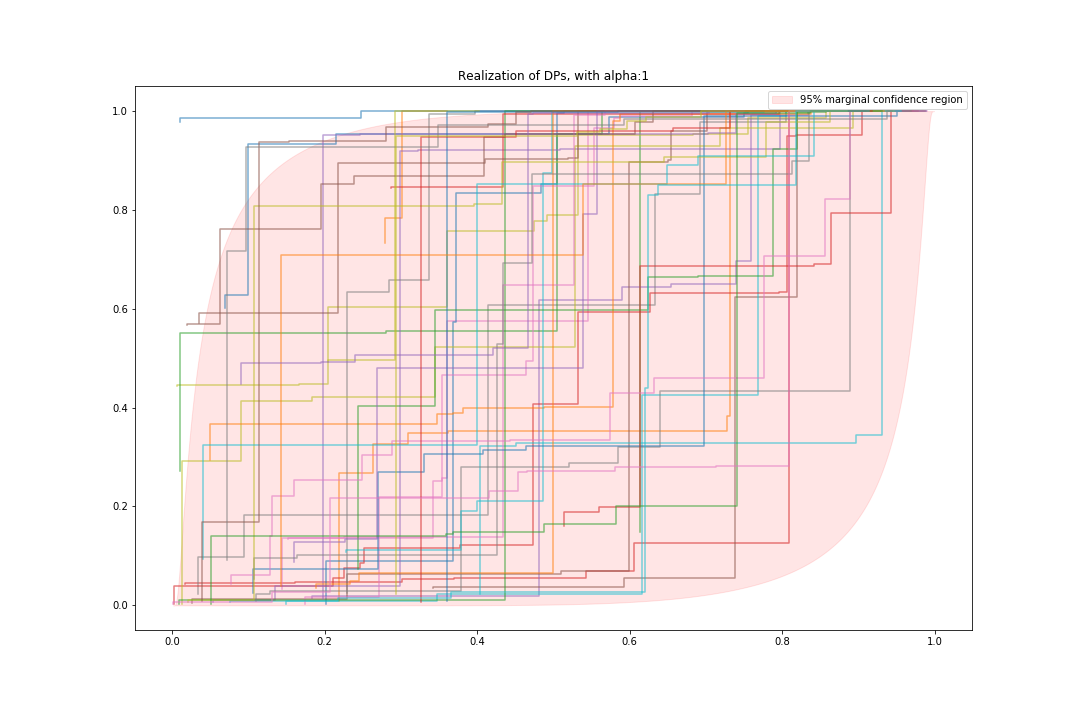
\includegraphics[width=0.5\linewidth]{DP1.png}\hfill
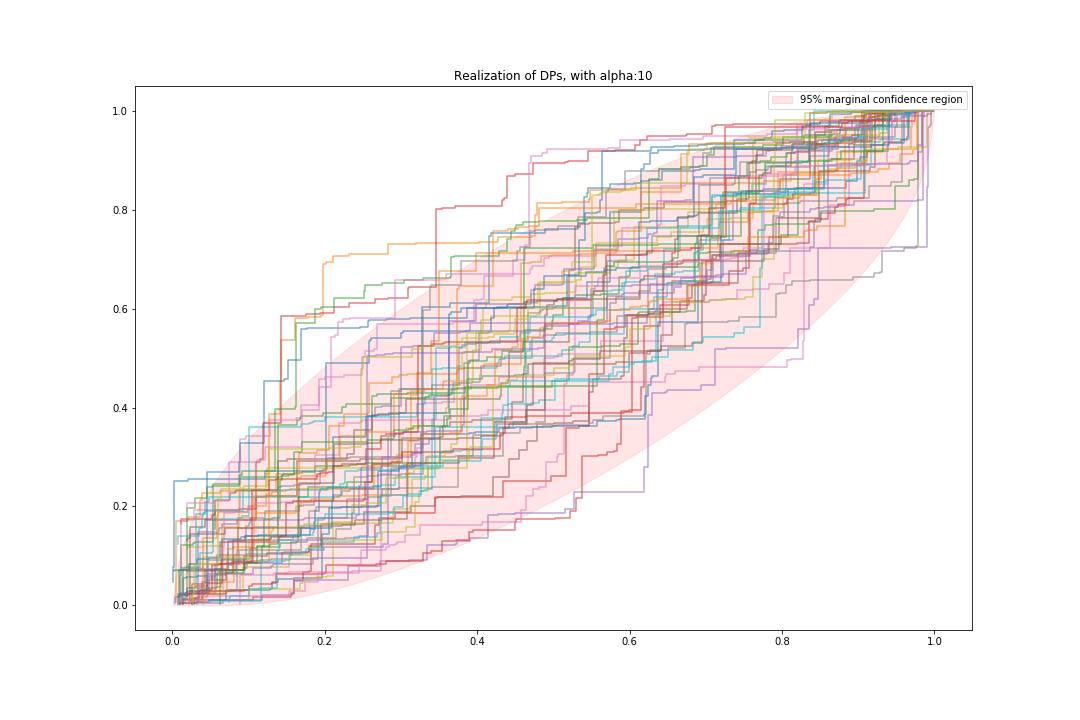
\includegraphics[width=0.5\linewidth]{DP_alpha=10.png}\hfill
 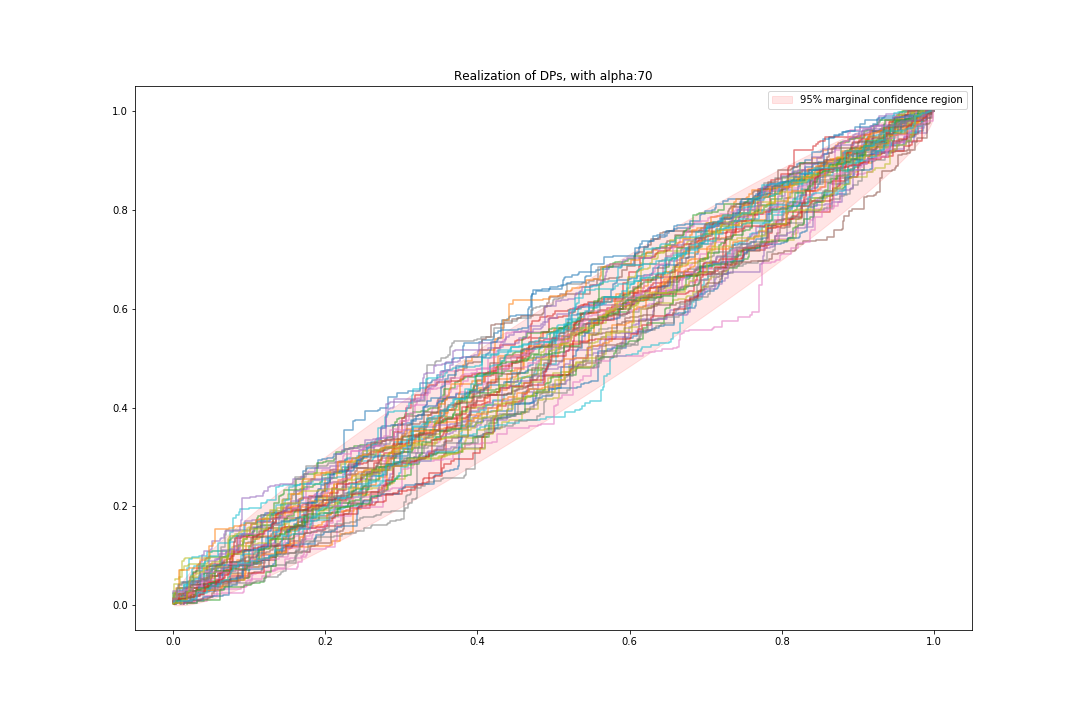
\includegraphics[width=0.5\linewidth]{DP_alpha=70.png}\hfill
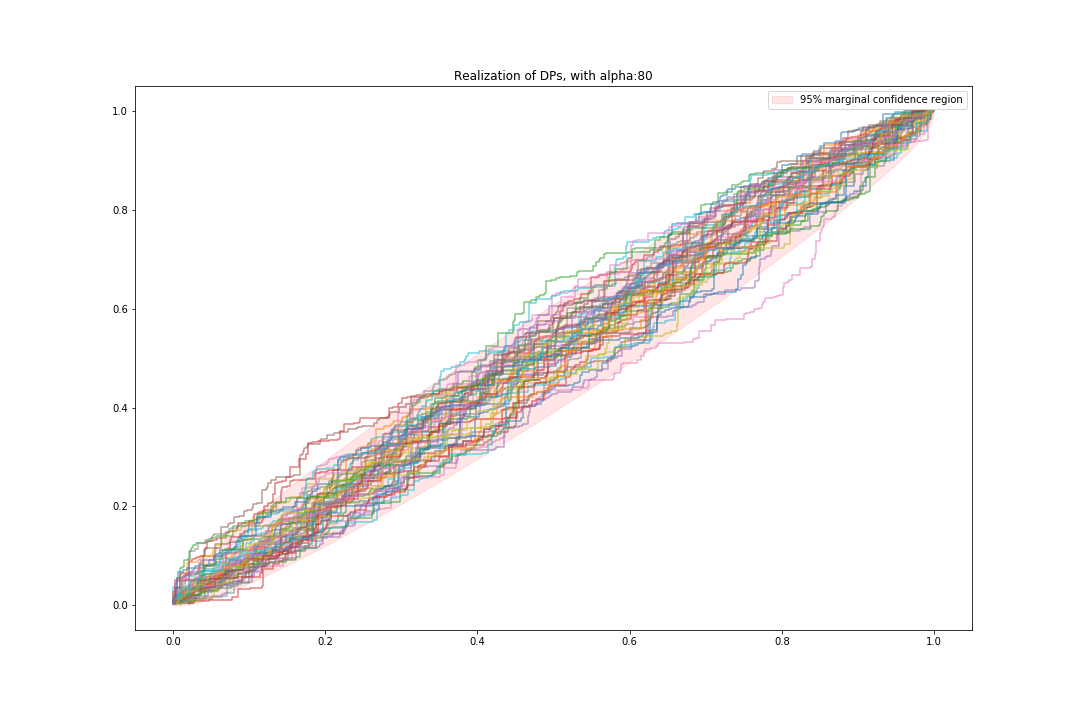
\includegraphics[width=0.5\linewidth]{DP_alpha=80.png}
\end{minipage}
\caption{Comparing the empirical distribution functions of the $\mathcal{DP}(\alpha, P_0)$ for $alpha=1, 10, 70, 80$. In shaded pink we signal the 95-percent exact confidence bands given by $\eqref{f(t)}$ }
\end{figure}


As we can see from the first set of figures, when we increase the value of $alpha$, the trajectories of the $\textit{Dirichlet Process}$ become more concentrated around the base measure $P_0$, which in our case is the $U(0,1)$.

Furthermore, it could be also interesting to study the behaviour of such a model when there actually exists a true data generating model. Indeed, from what said above, we already know that:

$$ DP(\alpha, P_0 | y_1,..., y_n) \sim DP(\alpha+n, \frac{\alpha}{\alpha+n} P_0+ \frac{1}{\alpha} \sum \delta_{y_i}).$$
A the question one should ask himself is whether such a posterior somehow converges to the true data generating distribution whenever we have infinite data at our disposal. The answer is positive, and it's clear looking at the form of the posterior: we will keep sampling from the old values with high probability (the ones coming from the "true" data generating) and almost never from our arbitrarily chosen base measure.

We report below some graphs of the trajectories of the posterior distributions computed with data coming from a standard Cauchy, highlighting the true $\textit{cdf}$ and the one of the base measure. Simulations are done for different values of $\alpha$ (1 and 10) and different sample size of the true data (10 and 100). Confidence bands are drawn also for this case.
As expected, the value of $\alpha$ becomes less and less relevant the more data we have (the two graphs on the left comes from $\alpha=1$, the one on the left for $\alpha = 10$). Furthermore, with larger $n$, the posterior distribution becomes more concentrated around the true data generating function, as its visible in the graphs below (upper graphs have $n=10$, lower ones $n=100$).

\begin{figure}[H]
\label{f2}
\begin{minipage}{1\textwidth}
%\centering
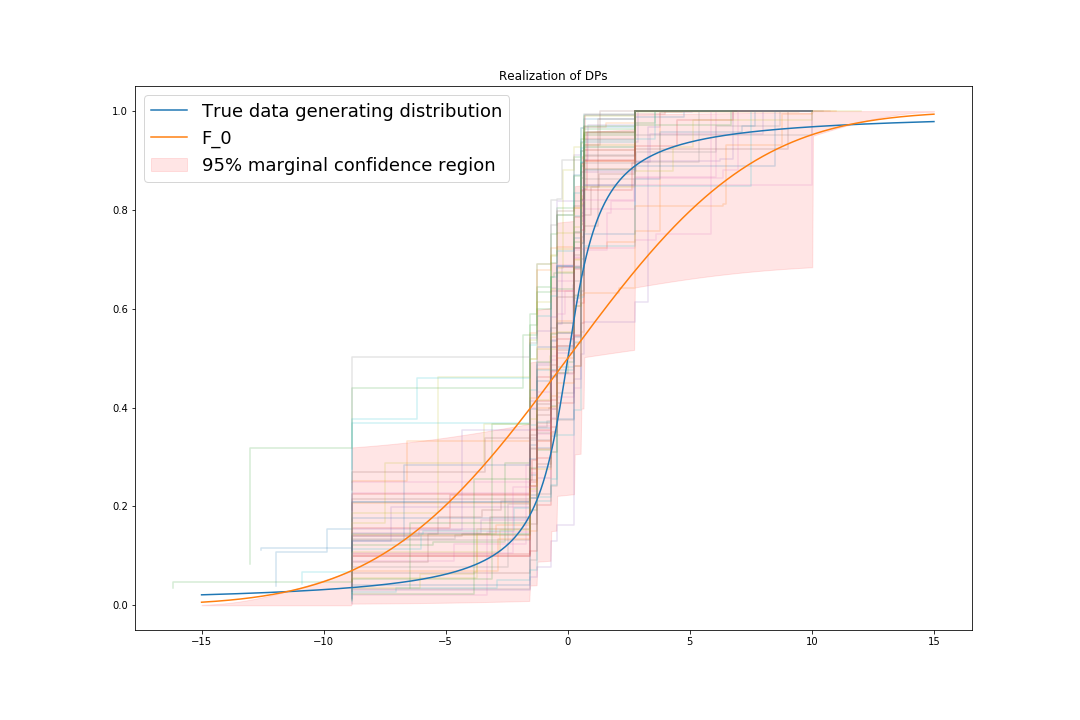
\includegraphics[width=0.5\linewidth]{DP_posterior10_1.png}\hfill
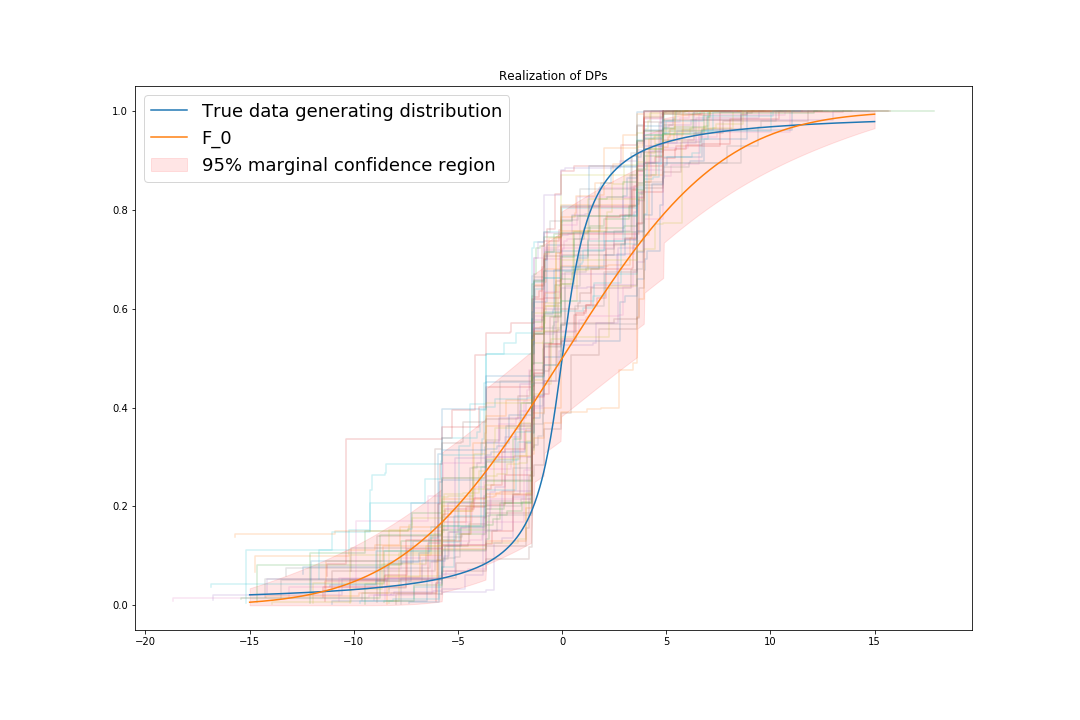
\includegraphics[width=0.5\linewidth]{DP_posterior10_10.png}\hfill
\includegraphics[width=0.5\linewidth]{DP_posterior100_1.png}\hfill
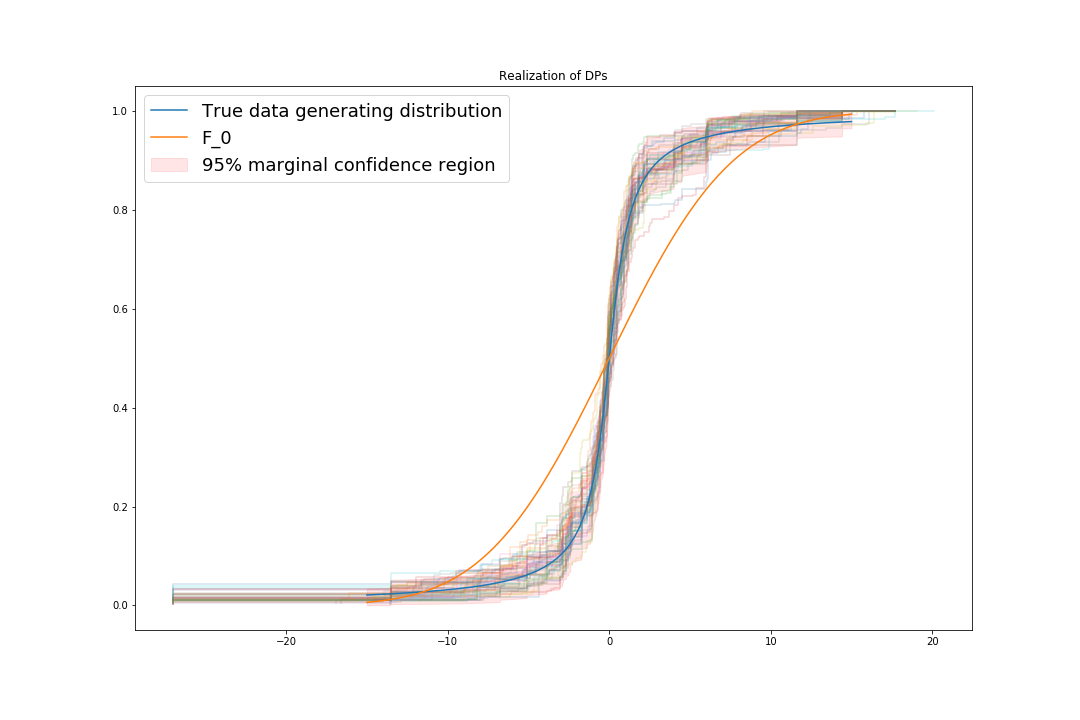
\includegraphics[width=0.5\linewidth]{DP_posterior100_10.png}
\end{minipage}
\caption{Comparing the trajectories of the posteriors} 
\end{figure}

\end{document}
